\documentclass[twocolumn,superscriptaddress,aps,prb,floatfix]{revtex4-1}

\usepackage{graphicx}% Include figure files
\usepackage{dcolumn}% Align table columns on decimal point
\usepackage{bm}% bold math
\usepackage{color}
\usepackage[caption=false]{subfig} 

\usepackage{listings}

\definecolor{dkgreen}{rgb}{0,0.6,0}
\definecolor{gray}{rgb}{0.5,0.5,0.5}
\definecolor{mauve}{rgb}{0.58,0,0.82}

\lstset{frame=tb,
  language=python,
  aboveskip=3mm,
  belowskip=3mm,
  showstringspaces=false,
  columns=flexible,
  basicstyle={\small\ttfamily},
  numbers=none,
  numberstyle=\tiny\color{gray},
  keywordstyle=\color{blue},
  commentstyle=\color{dkgreen},
  stringstyle=\color{mauve},
  breaklines=true,
  breakatwhitespace=true,
  tabsize=3
}

\usepackage{amsthm}
\usepackage{amsmath}
\usepackage{amssymb}

\newcommand{\Htc}{H_{\mathrm{TC}}}
\newcommand{\figref}[1]{Fig. \ref{#1}}


\newtheorem{theorem}{Theorem}[section]
\newtheorem{lemma}[theorem]{Lemma}
\newtheorem{proposition}[theorem]{Proposition}
\newtheorem{corollary}[theorem]{Corollary}

%\newenvironment{proof}[1][Proof]{\begin{trivlist}
%\item[\hskip \labelsep {\bfseries #1}]}{\end{trivlist}}
%\newenvironment{definition}[1][Definition]{\begin{trivlist}
%\item[\hskip \labelsep {\bfseries #1}]}{\end{trivlist}}
%\newenvironment{example}[1][Example]{\begin{trivlist}
%\item[\hskip \labelsep {\bfseries #1}]}{\end{trivlist}}
%\newenvironment{remark}[1][Remark]{\begin{trivlist}
%\item[\hskip \labelsep {\bfseries #1}]}{\end{trivlist}}

%\newcommand{\qed}{\nobreak \ifvmode \relax \else
%      \ifdim\lastskip<1.5em \hskip-\lastskip
%      \hskip1.5em plus0em minus0.5em \fi \nobreak
%      \vrule height0.75em width0.5em depth0.25em\fi}

\begin{document}

%\allowdisplaybreaks

\title{Finite temperature thresholds in the toric code with few measurements}


\author{C. Daniel Freeman}
\email{daniel.freeman@berkeley.edu}
\affiliation{Berkeley Quantum Information \& Computation Center, University of California, Berkeley, CA 94720, USA}
\affiliation{Department of Physics, University of California, Berkeley, CA 94720, USA}

\author{C. M. Herdman}
\affiliation{Institute for Quantum Computing, University of Waterloo, Waterloo, ON N2L 3G1, Canada}
\affiliation{Department of Chemistry, University of Waterloo, Waterloo, ON N2L 3G1, Canada}
\affiliation{Department of Physics \& Astronomy, University of Waterloo, Waterloo, ON N2L 3G1, Canada}

\author{K. B. Whaley}
\affiliation{Berkeley Quantum Information \& Computation Center, University of California, Berkeley, CA 94720, USA}
\affiliation{Department of Chemistry, University of California, Berkeley, CA 94720, USA}

\date{\today}

\begin{abstract}
 We prove the existence of a finite temperature threshold in the toric code in the absence of measurement of all stabilizers per error correction cycle.  Additionally, we leverage this proof to define a protocol that significantly extends the lifetime of the toric code which uses a sub-extensive number of measurement operators per error correction cycle.  Specifically, as system size, $N$, is made large, the number of requisite measurements grows only as $\sqrt{N} \rm{log}N$.   
\end{abstract}

\maketitle


%%%%%%%%%%%%%%%%%%%%%%
%%%%%%%%%%%%%%%%%%%%%%
\section{Introduction}
\label{sec:Intro}
%%%%%%%%%%%%%%%%%%%%%%

 While an ideal finite temperature quantum memory would require no active error correcting elements, no such systems are known to exist in an experimentally accessible number of dimensions.  Practically, the operation of a quantum memory is a balance between passive elements (i.e. dissipative cooling), and active measurement and correction cycles to keep quantum information protected.  In previous work, we analyzed the finite temperature dynamics of the toric code, verifying the well-known no-go theorems for the upper bound to the lifetime of the toric code at finite temperature.  Using this analysis, we were able to construct a measurement-free protocol for protecting the encoded qubits of the toric code, but these protocols again were limited by the no-go theorems, and only provided a multiplicative constant increase to the lifetime.  
 
 In this work, we examine the extent to which a limited amount of measurement can increase the lifetime of the toric code.  In sum, we prove that, for any constant density of measurements for a toric code undergoing dissipation at a fixed temperature, a threshold can be achieved.  Further, we provide an additional protocol with asymptotically vanishing density of measurements that provides an enhancement to the lifetime up to a temperature dependent cutoff.
	
%%%%%%%%%%%%%%%%%%%%%%
\section{The Toric Code at Finite Temperature}
\label{sec:TORIC}

\subsection{Definitions}
\label{sec:Defs}
%%%%%%%%%%%%%%%%%%%%%%
In this section, we briefly review the theory of the toric code, as well as the Lindblad formalism for evaluating its finite temperature dynamics.

\begin{align}
\Htc &= -J_e \sum_v A_v -J_m \sum_p B_p ,\label{eq:HTC}\\
A_v &\equiv \prod_{j \in v} \sigma_j^z,\quad B_p \equiv \prod_{j \in p} \sigma_j^x,\label{eq:AvBp}
\end{align}

\subsection{Finite Temperature vs. Infinite Temperature}
\label{sec:temperature}

 The vast majority of the error correction literature assumes an error model akin to an ``infinite temperature limit''.  More precisely, an array of qubits receives an error from some set of error operators ${E_i}$ independently at random with some probability $p$ every error correction cycle.  The threshold theorems state that there exists some critical error probability $p_c$ below which it is possible to return an error correcting code to its encoded state with unit probability for asymptotically large systems.  For the toric code, $p_c\approx.11$.
 
 Contrariwise, thresholds at finite temperature are usually quoted in terms of a critical \emph{temperature}.  That is, there must exist some critical temperature $T_c$ below which codes can be reliably corrected.  Unfortunately, this definition obscures a great deal of physics---different choices of bath model can greatly affect the dynamics of the error processes, to the extent that a quoted ``critical temperature'' often implicitly specifies a choice of bath.  Because different bath interactions can give rise to different system dynamics, the choice of bath also directly affects the strategy used for error correction.  Thus, to be as clear as possible, we choose here to treat the toric code undergoing dissipation by coupling to an Ohmic bath.

 Operationally, the choice of bath affects the system dynamics through the spectral density, $J(\omega)$. 


%%%%%%%%%%%%%%%%%%%%%%
%%%%%%%%%%%%%%%%%%%%%%
\section{Measurement Thresholds}
\label{sec:measurement_threshold}
%%%%%%%%%%%%%%%%%%%%%%

\subsection{Proof for Constant Measurement Density}

 It is well known that for total measurement density $m=1$, a threshold exists for the toric code.  Here we provide a proof for the existence of a threshold for any $m>0$ provided the toric code undergoes dissipation as described in \ref{sec:temperature}.  Specifically, below a finite temperature $T_c$, which we will explicitly lower bound as a function of the measurement density $m$, the measurement rate $\chi_{\rm{M}}$, and a unitary application rate $\chi_{U}$, it will be possible to return the toric code to its encoded state with unit probability in the large system size limit.  First, we review the $m=1$ case to further clarify the differences between finite temperature error correction and the usual ``infinite temperature'' limit.
 
 \subsubsection{Complete Measurement}
 
  In the infinite temperature case, errors are applied independently at random to all of the qubits of the toric code each error correction cycle.  This is identical to the Ohmic ``infinite temperature'' case where $\gamma_+ / \gamma_- = \gamma_+ / \gamma_0 = 1$.  These choice of rates ensures that pair-creation, pair-annihilation, and translation occur at the same rate, effectively causing errors to occur with equal probability on every edge.  To make the correspondence precise, the measurement rate must be chosen so that some fixed number of system bath interactions $N_c$ happens on average every measurement cycle.  For a measurement rate $\chi_{\rm{M}}$, this is satisfied if $\chi_{\rm{M}} = N_c \gamma_+$.  Then, the analogue of the error probability per edge is given by $p = \frac{N_c \gamma_+}{2L^2}$.
 
  At non-``infinite'' finite temperature, we can classify the different regimes based on two qualities: average number of defects and speed of defects.  Generically, the faster defects move (i.e., the larger $\gamma_0 / \gamma_+$), the more difficult error correction becomes.  Likewise, the higher the average number of defects relative to the total number of sites, the more difficult to correct errors.  A ``phase diagram'' of correctability is depicted in \figref{fig:errorphase}.
  
  We will treat two limits here explicitly: $(1)$ fast defects with low average number, and $(2)$ slow defects with high average number.

 $(1)$: For $O(1)$ defects in the system on average, the code is correctable so long as any single defect pair does not become separated by $L/2$ sites.  Because the motion of the defects is diffusive, and because the timescale for a single translation event is $1/\gamma_0$, the timescale over which these uncorrectable excursions occur (conditioned on a free pair of defects being in the system) is $(1/\gamma_0) (L/2)^2$.  Thus, for any measurement rate $\chi_{\rm{M}}$, simply by scaling the lattice sufficiently large, these defects can be corrected with certainty.
 
 $(2)$: ``Slow'' defects can be idealized as the $\gamma_0\rightarrow 0$ limit, which is natural for Superohmic baths.  Here, the usual Nishimori line construction fails because the distribution of defects is not independent.  The precise effect of this is difficult to calculate, as it relies on the nonequilibrium dynamics of defects with interactions.  Namely, some edges feel an infinite ``excluded volume'' interaction that prevents an error from occuring on a given edge $e$ unless an even number of adjacent edges also have errors.  In the dual quasiparticle picture, this is equivalent to the condition that defect pairs can only be created or destroyed---not translated.
  
 
 
 \subsubsection{Incomplete Measurement}
 
  Naively, at ``infinite temperature'', error correction can occur so long as defects can be shuttled onto the measurement operators sufficiently rapidly.  That is to say, one could imagine instead of measuring the entire lattice, first dividing the lattice into regions of size $L^2 m$ and measuring one such region each cycle.  After $\rm{ceil}(1/m)$ cycles, one would have measured the entire lattice, and if the cycle were short enough relative to the timescale over which errors occur, could correct errors with certainty.
 
 This strategy is suboptimal for a variety of reasons.  First, it supposes that measurements can either be made in principle everywhere, which may not be true due to hardware constraints, or that the resources exist to shuttle defects onto fixed measurement sites.  For fixed measurement resources---i.e., a fixed number of vertices where measurement can occur---one would have to perform swapping operations to shuttle possibly unmeasured defects onto the measurement operators.  The number of swaps necessary grows quartically with $1/m$  Additionally, if measurements can be made on all sites, there's no reason \emph{not} to measure \emph{all} the stabilizers every corrective cycle.  For the following analysis, then, we will assume that the measurement resources are in a fixed geometry.

 Regardless, this naive strategy sets an upper bound to how quickly measurements must occur to provide error correction.  If errors occur independently at random on average every $\tau$, then $\frac{1}{m \chi_{\rm{M}}} \leq p_c 2L^2 \tau$, where $p_c\approx.109$.  This inequality simply states that the timescale associated with measurement of all the vertices must be less than or equal to the timescale associated with the critical fraction of the lattice receiving errors.
 
 Without loss of generality, consider the pattern of measurement operators in figure \figref{fig:MeasurementScaling}.  Intuitively, this pattern of measurements sequesters the lattice into regions of characteristic area $L^2 / (mL/2 + 1)^2 \:= a_{\rm{M}}$.
 

 
\begin{figure}
\begin{center}
\scalebox{1}{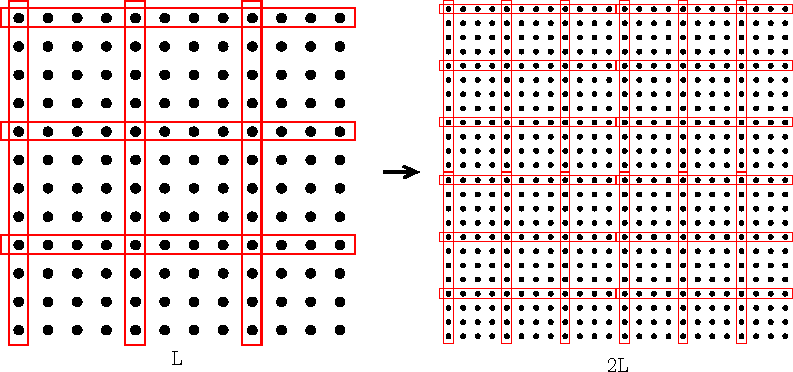
\includegraphics[width=1.0\columnwidth]{MeasurementScaling}}
\end{center}
\caption{Toric code vertices (in black) with pattern of vertices chosen for measurement (boxed in red).  On the left is a pattern of measurements for a system of characteristic edge length $L$.  On the right is a pattern for a system with edge length $2L$.  Note the fraction of measured vertices to total vertices (i.e., $m$) remains fixed.}
\label{fig:MeasurementScaling}
\end{figure}

 Suppose that every vertex stabilizer indicated in \figref{fig:MeasurementScaling} is measured every measurement cycle, and that measurement cycles occur with rate $\chi_{\rm{M}}$.  Choose the temperature $T$ such that $a_{\rm{M}} \gamma_+ = .01.$  This choice is not unique, and is only chosen to guarantee the expected number of defects in any given region of size $a_{\rm{M}}$ is much less than one.  On any given measurement cycle, there is no hope of performing error correction unless the measurement rate $\chi_{\rm{M}}$ is much faster than the intrinic defect hopping rate $\gamma_0$.  To allow a concrete estimate, suppose $\gamma_0/\chi_{\rm{M}}=.01$.
 
 Finally, suppose that, on detection of a defect, there exists a protocol that will efficiently encourage dissipation with the measured defect and a possibly unmeasured pair (without further measurement) which possesses a constant failure probability $p_f=.01$.  We provide such a protocol in the Appendix.
 
 To upper bound the error rate, we will make several crude approximations.  First, we assume that defects ballistically separated by more than 1 vertex.  Then, a crude estimate for the number of trajectories with total defect separation $|v_i - v_j|$ (taxicab norm) is 
 
 




\bibliography{manuscript_TC_2}

\end{document}
%
% ****** End of file apssamp.tex ******

%\begin{align}
%D^\dagger_{b}&= \frac{1}{4} \left(I  \sigma_x  I + \sigma_z  \sigma_x  \sigma_z + i \left(I  \sigma_y  \sigma_z + \sigma_z  \sigma_y  I \right) \right), \notag \\ 
%D_{b}&= \frac{1}{4} \left(I  \sigma_x  I + \sigma_z  \sigma_x  \sigma_z - i \left(I  \sigma_y  \sigma_z + \sigma_z  \sigma_y  I\right)\right), \notag \\
%T_{b}&=\frac{1}{2} \left(I  \sigma_x  I - \sigma_z  \sigma_x  \sigma_z \right) \label{eq:LindbladDef}
%\end{align}
